\chapter{Overview of the Indian Summer Monsoon}
\label{c:ism_overview}
The Indian Summer Monsoon is a global climatic phenomenon that has been actively researched for decades. Even though many theories and hypotheses exist, the factors influencing its strength, timing and variability have still not been fully identified and understood. This chapter aims to provide a short overview of the observed behavior and current scientific understanding of ISM, as far as the foreknowledge might prove useful for the further parts of this work.


\section{Seasons \& Progression}
\label{st:ism_seasons}
The ISM progresses over the Indian subcontinent in three main phases: the pre-monsoon season (March-May), the primary monsoon season (June-September) and the post-monsoon season (October-December) \citep{Stolbova.2015}.

The months of the pre-monsoon season correspond to the Indian summer and are characterized by high temperatures with low amounts of rainfall over regions in the Himalayas and south-west India. Many predictions about the further development of ISM are commonly based on the pre-monsoon season, especially on the patterns that occur leading up to the primary monsoon season \citep{Stolbova.2015}.

A sudden transition with rapidly increasing amounts of daily rainfall, moisture, and kinetic energy, as well as increased vertical shear in horizontal winds\footnote{A gradient between wind speeds at different heights or pressure levels.}, then marks the beginning of the primary monsoon season \citep{Pradhan.2017}. This transition, the "onset" of monsoon, occurs at different times for different parts of the Indian subcontinent, as can be seen in \cref{fig:onset_propagation}. First arriving in Kerala on the southwestern tip of the subcontinent around the first of June, the ISM then propagates north- and northwestwards, where it reaches the Pakistani border around the 15th of July \citep{Willetts.2017}.

\begin{figure}[h]
  \centering
  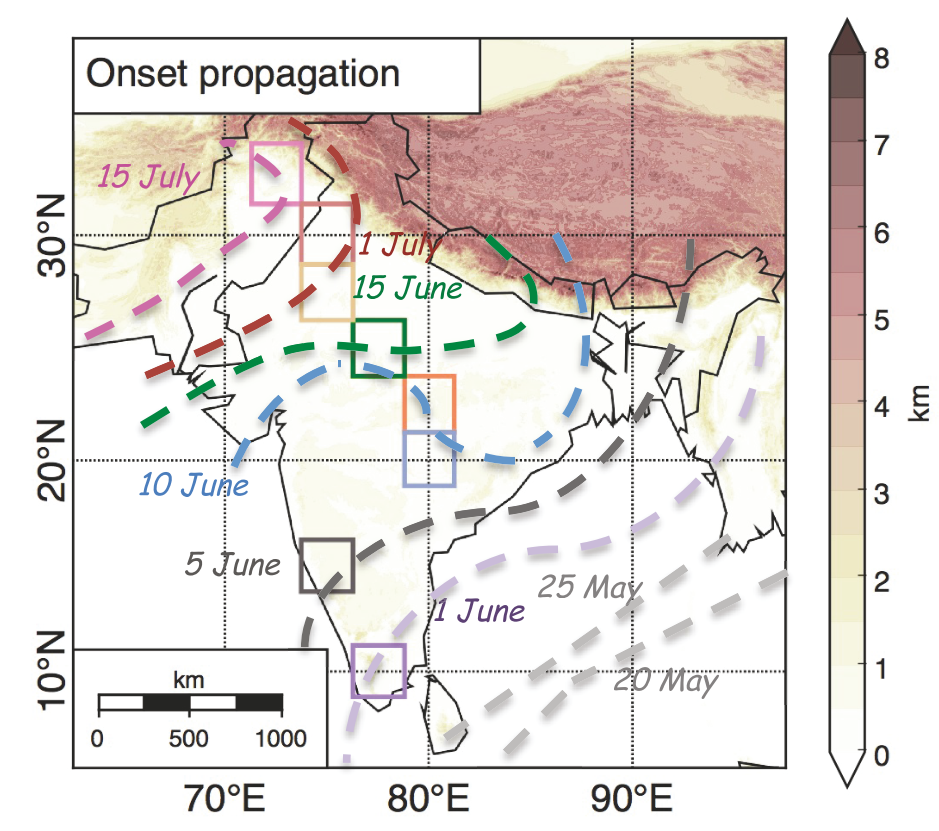
\includegraphics[width=0.45\linewidth]{./99_appendix/img/stolbova_propagation}
  \caption{Propagation of monsoon over the Indian subcontinent as depicted in \citet{Stolbova.2015}, based on a recreation of the official figure by the IMD.}
  \label{fig:onset_propagation}
\end{figure}

After the ISM has fully covered the Indian subcontinent in July, most places experience its weather conditions well into September. When the monsoon starts its retreat from northern India, its progression reverses, and it gradually withdraws from the subcontinent, entirely leaving the subcontinent in October.

During the post-monsoon season, parts of the Indian subcontinent experience a second extended period of rainfall called the \textit{North-East Monsoon}. Some places in north-eastern India receive more rainfall during the North-East Monsoon than during the primary season of the ISM. This work is, however, focused mostly on the Indian Summer Monsoon, because of which we will not be covering the North-East Monsoon in more detail.


\section{Main Drivers}
\label{st:ism_factors}
In its most basic form, the ISM can be seen as a sea breeze of enormous extent. The hot summer weather during the pre-monsoon season causes a heating of the Indian subcontinent. An increasingly large temperature gradient due to slower heating of the Indian Ocean then causes air to flow onto the subcontinent, bringing with it the moisture necessary to cause precipitation \citep{Willetts.2017}.

Intense heating and heat dissipation of the high-altitude Tibetan Plateau lead to an increase in the tropospheric temperature, creating an area of low-pressure near the surface that attracts moisture from surrounding areas over the Indian Ocean \citep{Stolbova.2015}. The low-pressure zone further causes strong vertical air currents from south of the Tibetan Plateau, aiding the ISM with its propagation into the far north of India \citep{Pradhan.2017}.

On a larger scale, the ISM has been linked to several parts of the global atmospheric circulatory system. A shift of the subtropical jet stream to the north of the Tibetan Plateau as well as interaction with the westerly jet stream have been found to influence the behavior of the ISM \citep{Ordonez.2016, Stolbova.2015}. A strong westerly jet in the lower troposphere over Kerala seems to correlate with the monsoon onset of the region \citep{Ordonez.2016}. Additionally, the Somali jet passing over the Arabian sea cools down the body of water, further strengthening the temperature gradient \citep{Stolbova.2015}.

The trade winds of the northern and southern hemisphere meet to create the Intertropical Convergence Zone (ITCZ), a belt of low-pressure close to the thermal equator. When the ITCZ moves north following the summer months, it further increases the variability of weather events and thus reduces their predictability \citep{Stolbova.2015}.

A further factor in the development and strength of the ISM is the El Niño Southern Oscillation (ENSO). The warming of the Humboldt ocean current during El Niño years causes the land-ocean temperature gradient to decrease. This tends to decrease the amount of rainfall the Indian subcontinent receives and can delay the onset of monsoon by several days \citep{Pradhan.2017, Willetts.2017}. Conversely, the cooling of the current during La Niña can result in more rainfall and an earlier onset due to a higher temperature gradient.

A combination of the factors above creates a low-pressure channel (a ``monsoon trough'') closely south of and parallel to the Tibetan Plateau that serves as a primary source of moisture during the ISM \citep{Stolbova.2015}.

The World Meteorological Organization (WMO) describes the ISM as only part of a global monsoon system, by which it is interlinked with other monsoon regions all over the world \citep{WorldMeteorologicalOrganization.2005}. The ISM as described is part of a larger Asian monsoon system, which additionally includes the \textit{East Asian Summer Monsoon (EASM)} and the \textit{Western North Pacific Summer Monsoon (WNPSM)}, as is shown in \cref{fig:monsoon_system} \citep{Yihui.2005}. While the ISM has been the focus of monsoon research for decades, the theory of a global circulatory monsoon system has been investigated for a much shorter period \citep{WorldMeteorologicalOrganization.2005}. As such, much about the global teleconnections between different regional monsoon systems is still unknown.

\begin{figure}[h]
  \centering
  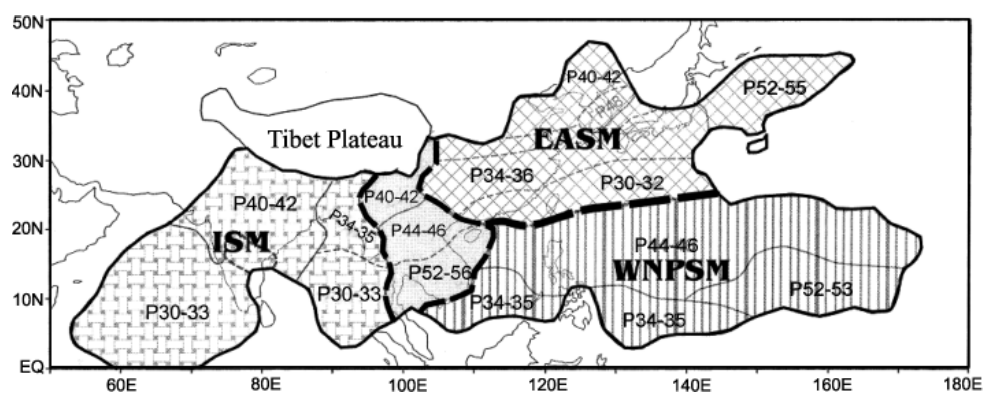
\includegraphics[width=0.55\linewidth]{./99_appendix/img/monsoon_system}
  \caption{Monsoon system over Asia as found in \citet{Yihui.2005}.}
  \label{fig:monsoon_system}
\end{figure}

This summarization of the impacting factors of the ISM is not exhaustive, as the ISM is much more complex and some of its behavior and teleconnections have still not been fully explained. However, knowledge of these fundamental factors should already provide a good intuition for \cref{c:event_sync} and \cref{c:part2}.


\section{Trends}
\label{st:ism_trends}
Much like the global climate, the ISM is exposed to trends that can impact its variability and predictability. A major trend that was prevalent during the second half of the 20th century was a decrease in monsoon rainfalls over northern-central India close to the Tibetan Plateau \citep{Jin.2017}. One theory states that such a drying trend could be connected to a warming of the surrounding Indian Ocean. A resulting weakening of the land-ocean temperature gradient could have been responsible for the lower rainfall amounts. A further hypothesis states that large-scale deforestation could have decreased the amount of transpiration from plants, resulting in less moisture and thus precipitation \citep{Jin.2017}.

In addition to the weakening precipitation, it has been found that the frequency of heavy and extreme rainfall events increased by 50\% and 100\% respectively. At the same time, short and long dry spells were found to occur increasingly often \citep{Auffhammer.2012}. The drought during the 2009 monsoon season was more severe than most that occurred in the previous decades \citep{Auffhammer.2012}. As such, the overall trend seems to be an increase in general extremes, be it extreme rainfall or no rainfall at all.

Surprisingly, \citet{Jin.2017} have found that the precipitation weakening trend has reversed for most parts of India after 2002, which is also shown in \cref{fig:precipitation_trend}. The reversal is attributed to changing trends of features like the temperature gradient between land and sea temperature during the pre-monsoon season, which, since 2002, is increasing at both a surface level and in the mid-troposphere, while it was decreasing beforehand \citep{Jin.2017}.

\begin{figure}[h]
  \centering
  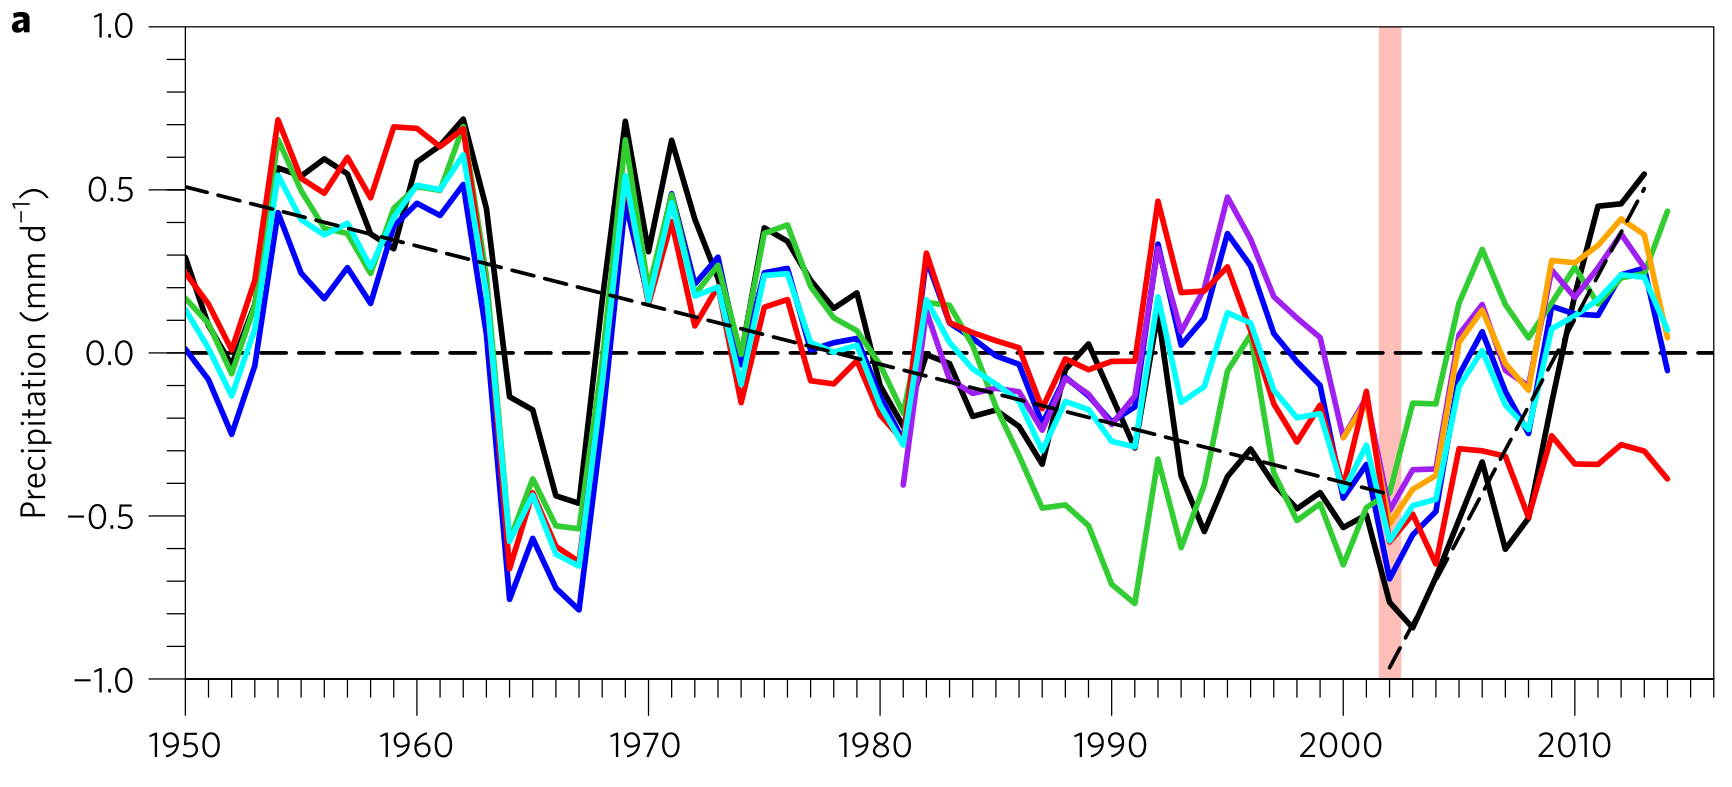
\includegraphics[width=0.7\linewidth]{./99_appendix/img/precipitation_trend}
  \caption{Trends of various precipitation datasets as depicted in \citet{Jin.2017}. The TRMM dataset is represented by the orange line.}
  \label{fig:precipitation_trend}
\end{figure}


\section{Social Impact}
\label{st:ism_impact}
As we have already seen, the ISM is one of the most impactful large-scale meteorological events on earth. It affects the lives of up to one-fourth of the world's population: the people living on and around the Indian subcontinent \citep{Stolbova.2015}. The heavy rainfalls that the ISM brings with it are of great importance for the population in India and many of its surrounding countries.

Livelihood on the Indian subcontinent is strongly coupled to a timely occurrence of the ISM. Monsoon rainfalls are responsible for 80 percent of the annual precipitation on the Indian subcontinent \citep{Jin.2017}. Farmers depend on these rainfalls to water their crops and feed their livestock. Up to 2012, more than half of a year's rice harvest was still grown during the monsoon period \citep{Auffhammer.2012}. The agricultural sector accounts for almost one-fifth of India's GDP, and about 50\% of the population in India either directly or indirectly depend on the agricultural sector \citep{CentralIntelligenceAgency.05.01.2018}, making the ISM equally important for the economy as a whole. Historically, years with sub-par monsoon rainfalls or even droughts have caused massive losses for farmers as well as high reductions in the general economy and welfare. For example, the heavy drought in 2009 caused the rice harvest to decrease by 14\% \citep{Auffhammer.2012}.

The apparent impactfulness of the ISM makes clear the need of being able to predict the monsoon behavior and its onset and withdrawal dates accurately. If farmers knew in advance when monsoon rainfalls would start and how long they would last, they could wait until the appropriate time to plant their crops. On the contrary, if they get surprised by either early or late onset of monsoon or even drought-like conditions, their crop yield might be reduced, or their crops destroyed entirely. Reliable predictions are thus highly called for, as they could reduce these risks as well as general concerns about food security. Furthermore, with the increasing trend in extreme events on both sides of the scale, analyzing their spatial distribution poses an interesting research question. It is probable that the occurrence of extreme events adheres to some patterns, the understanding of which could help mitigate risks of floods or landslides.
